\title{One-dimensional clustering with one cluster}

\begin{abstract}
	The simplest case of clustering is the one dimensional case:
	when we want to find clusters of a given set of numbers.  The
	simplest 1D clustering is when we know that there is only a
	single cluster.  This document is a comprehensive study of
	this simplest case.  Namely, given a finite set of real
	numbers that form ``one cluster'', we explain how to find it;
	that is how to determine its position and its size.  This
	problem has actually many solutions with very different
	properties, and we try to cover them all.
\end{abstract}

\newcommand{\R}{\mathbf{R}}
\newcommand{\Z}{\mathbf{Z}}

\section{The Pythagorean means and the median}

Our goal is to combine a set of~$N$ numbers~$x_1,\ldots,x_N$ into a
single one.  The simplest choice is the~\emph{average}, also
called~\emph{arithmetic mean}:
\[
	\mathrm{avg}(x_1,\ldots,x_N) := \frac{x_1+\cdots+x_N}{N}
\]
We also have the harmonic mean:
\[
	\mathrm{har}(x_1,\ldots,x_N) :=
	\frac{N}{\frac{1}{x_1}+\cdots+\frac{1}{x_N}}
\]
and the geometric mean:
\[
	\mathrm{geo}(x_1,\ldots,x_N) :=
	\sqrt[N]{x_1\cdot \cdots\cdot x_N}
\]
The geometric mean is somewhat different, because it is only
well-defined (as a function~$\R^N\to\R$ with arbitrary~$N$)
when all the numbers are positive.  As we will see, the harmonic mean
also really makes sense only when all the numbers are strictly positive.
However, the arithmetic mean has good properties for arbitrary input
numbers (positive, negative, or zero).

For positive numbers, we also have the~\emph{quadratic mean}, also
called~\emph{root mean square error}:
\[
	\mathrm{rms}(x_1,\ldots,x_N) :=
	\sqrt{\frac{x_1^2+\cdots+x_N^2}{N}}
\]
These four functions are called~\emph{Pythagorean means} and they are
all of fundamental importance.  They are related by the following
inequalities:
\[
	\mathrm{min}
	\le \mathrm{har}
	\le \mathrm{geo}
	\le \mathrm{avg}
	\le \mathrm{rms}
	\le \mathrm{max}
\]
These inequalities are elementary to prove for~$N=2$, and the general
case is a standard exercise.

Finally, the last ``traditional'' aggregator is the~\emph{median},
which is computed by sorting the numbers from low to high, and taking
the middle one (if~$N$ is odd) or the average of the two middle
ones~(if~$N$ is even).
\[
	\mathrm{med}(x_1,\ldots,x_N):=
	\begin{cases}
		x_{{}_{(M)}} & \textrm{if~$N=2M+1$} \\
		&\\
		\displaystyle\frac{x_{{}_{(M)}}
		+ x_{{}_{(M+1)}}}{2}
			& \textrm{if~$N=2M$}
	\end{cases}
\]
where~$x_{(1)},\ldots x_{(N)}$ indicates the sorted
numbers~$x_1,\ldots,x_N$.  There is no general inequality
relationship between~$\mathrm{med}$ and~$\mathrm{avg}$, either one can be larger or
smaller, depending on the particular set of numbers.


\section{Axiomatic characterization}

A map~$f:\R^N\to\R$ with the following properties
is called an aggregator function:
\begin{itemize}
	\item[P0.]
		(Identity)
		$\qquad$
		$f(c,\ldots,c)=c$
	\item[P1.]
		(Symmetry)
		$\quad$
		$f(x_{\sigma_1},\ldots,x_{\sigma_N})=f(x_1,\ldots,x_N)
		\quad
		\forall\sigma\in\mathrm{S}_N$
	\item[P2.]
		(Monotony)
		$\quad$
		$(x_1,\ldots,x_N)\le(y_1,\ldots,y_N)
		\implies
		f(x_1,\ldots,x_N)\le f(y_1,\ldots,y_N)$
	\item[P3.]
		(Bracketing)
		$\quad$
		$\mathrm{min}(x_1,\ldots,x_N)
		\le f(x_1,\ldots,x_N)
		\le \mathrm{max}(x_1,\ldots,x_N)$
	\item[P4.]
		(Homogeneity)
		$f(\lambda x_1,\ldots,\lambda x_N)
		=\lambda\ f(x_1,\ldots,x_N)
		\quad\forall\lambda >0$
\end{itemize}

Notice that these properties may only be true on a subdomain
of~$\R^N$ where~$f$ is well-defined (typically, the positive
numbers).  Properties~$P0--P4$ are very natural, and a bit redundant;
for example you can prove identity from monotony and bracketing, etc.

The following properties~$P5--P7$ are more special and aggregator
functions may or may not have them:

\begin{itemize}
	\item[P5.]
		(Additivity)
		$\quad$
		$f(\lambda+x_1,\ldots,\lambda+x_N)
		=\lambda+f(x_1,\ldots,x_N)$
	\item[P6.]
		(Composability)
		$f\left(f(x_1,\ldots,x_P),\ldots,f(x_{P(Q-1)},\ldots,x_{PQ})\right)
		=f(x_1,\ldots,x_N)\quad\forall PQ=N$
	\item[P7.]
		(Continuity)
		$\qquad$
		$f:\R^N\to\R$ is continuous
\end{itemize}

\section{List of examples}

This list should contain {\bf all} the aggregator functions that I
know (whether they are useful or useless).  Many aggregator functions
belong to families that depend on a real-valued parameter, and for
extremal values of the parameter they give the min and the max.
Thus, all these aggregators can be interpreted as different,
data-guided interpolators between min and max.

\subsection{Power means~$M_p$}

The \emph{power means}~$M_p$ are defined only for strictly positive numbers:
\[
	M_p(x_1,\ldots,x_N):=\sqrt[p]{\frac{1}{N}\sum_{i=1}^Nx_i^p}
\]
Notice that~$M_p$ is well defined for~$p\neq0$.  We extend the
definition~of~$M_p$ to~$p=0,\pm\infty$ by taking limits.  The
resulting definition contains all the Pythagorean means, the minimum and
the maximum as particular cases:

\medskip

\begin{tabular}{c|c}
	power mean & meaning \\
	\hline
	$M_{-\infty}$ & minimum \\
	$M_{-1}$ & harmonic mean \\
	$M_0$ & geometric mean \\
	$M_1$ & arithmetic mean \\
	$M_2$ & quadratic mean \\
	$M_3$ & cubic mean \\
	$M_\infty$ & maximum \\
\end{tabular}

\medskip

Notice that as the parameter~$p$ goes from~$-\infty$ to~$\infty$, the
power mean~$M_p$ interpolates from the minimum to the maximum sample,
passing through the Pythagorean means at the values
points~$p=-1,0,1,2$.

Power means satisfy properties~$P0--P4$ over the positive numbers.
Although~$M_{-1}$ can be defined also for negative numbers, it fails
to satisfy the bracketing property, so it is not considered as such.

Except for the values of~$p=1,\pm\infty$, the power means do not
satisfy the additivity property~$P5$.  Thus, they are essentially
tied to the position of the zero in the real line.

On the other hand, the power means are composable ($P6$).

\subsection{Order statistics~$O_k$ and~$O_{\alpha}$}

The power means are not the only natural interpolation between min
and max; there is indeed a more natural one: the order statistics.

Given a set of~$N$ numbers~$x_1,\ldots,x_N$, they can always be
re-indexed so that
\[
	x_{(1)} \le x_{(2)} \le \cdots \le x_{(N)}
\]
Thus~$\max(x_1,\ldots,x_N)=x_{(N)}$
and~$\min(x_1,\ldots,x_N)=x_{(1)}$.  In functional notation, we
define
\[
	O_k(x_1,\ldots,x_N) := x_{(k)}
\]
for~$k=1,\ldots,N$.  This definition is extended to
real-valued~$k\in[1,N]$ by interpolating linearly between the
two closest integer values of~$k$.  In that case, we often use the
notation~$O_{\alpha}$ for~$\alpha\in[0,1]$, where~$k=(N-1)\alpha+1$.
This notation has the advantage of being independent of~$N$, so
that~$O_{\frac{1}{2}}$ is always the median.  The following table
lists other particular cases

\medskip

\begin{tabular}{l|l}
	order statistic & meaning \\
	\hline
	$O_0$ & minimum \\
	$O_{0.1}$ & first decile \\
	$O_{0.25}$ & first quartile \\
	$O_{0.5}$ & median \\
	$O_{0.75}$ & third quartile \\
	$O_{0.9}$ & ninth decile \\
	$O_1$ & maximum \\
\end{tabular}

\medskip

Order statistics can be defined for arbitrary numbers (positive,
negative and zero) and they have the additivity property P5, thus
they are position-invariant.  However, except for the min and the
max, they are not composable (P6).


\subsection{Histogram modes $H_{\varphi,\psi}$}

A simple yet very robust way to locate a cluster, especially when
there is a large number of points, is to build and histogram of the
data and find its mode (the position of the bin with higher amount of
samples).  This method has two parameters, the~\emph{frequency} of the bins,
and the~\emph{phase}
\[
	H_{\varphi,\psi}(x_1,\ldots,x_N) :=
%	\psi+\frac{1}{2}\varphi+\varphi\argmax_{k\in\Z}
	\psi+\frac{1}{2}\varphi+\varphi\mathrm{argmax}_{k\in\Z}
%	\sum_{i=1}^N\int_0^1
%	\delta\left(y+k+\frac{\psi-x_i}{\varphi}\right)\d y
	\sum_{i=1}^N\int_{\psi+k\varphi}^{\psi+(k+1)\varphi}
	\delta(x-x_i)\,\mathrm{d}x
\]
%\[
%	H_{\varphi,\psi}(x_1,\ldots,x_N) :=
%	\psi+\frac{1}{2}\varphi+\varphi\argmax_{k\in\Z}
%	\sum_{i=1}^N\int_0^1
%	\delta\left(y+k+\frac{\psi-x_i}{\varphi}\right)\d y
%%	\sum_{i=1}^N\int_{\psi+k\varphi}^{\psi+(k+1)\varphi}
%%	\delta(x-x_i)\d x
%%
%%	H_{\varphi,\psi}(x_1,\ldots,x_N) :=
%%	\psi+\varphi\left(\frac{1}{2}+\arg\max_k\,\biggl\lvert\{x_1,\ldots,x_N\}\cap[\psi+k\varphi,\psi+(k+1)\varphi]\biggr\rvert\right)
%%
%%\[
%%	H_{\varphi,\psi}(x_1,\ldots,x_N) :=
%%	\psi+\varphi\left(\ \frac{1}{2}
%%	+
%%	\arg\max_k
%%	\,
%%	\biggl\lvert
%%	[k,k+1]\cap\left\{
%%	\frac{x_i-\psi}{\varphi}
%%	\right\}_{i=1,\ldots,N}
%%	\biggr\rvert
%%	\ \right)
%\]
%where the vertical bars denote the cardinal of a finite set.
Notice
that the result depends on the two parameters~$(\varphi,\psi)$ in a
very beautiful and fractal way (see image below).
It is impossible to set reasonable values of these parameters without
knowing anything about the nature of the input data.

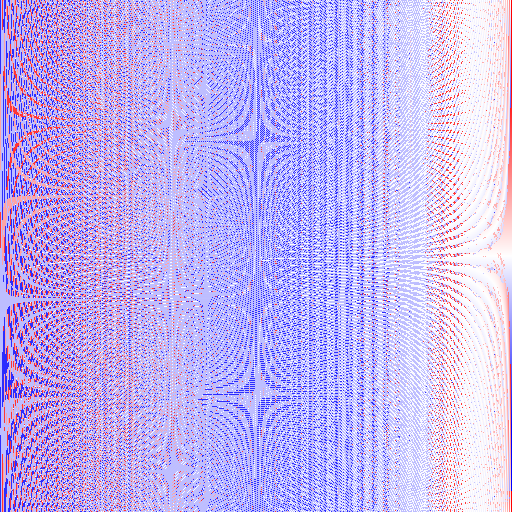
\includegraphics{i/modefractal.png}



\subsection{Fréchet $p$-centroids~$F_p$}

On a metric space~$(M,d)$, the Fréchet centroid of a set of
points~$p_i\in M$ is the point~$c\in M$ that minimizes the sum of
squared differences to~$p_i$
\[
	c := \mathrm{argmin}_{m\in\R}\sum_{i=1}^N d^2(p_i,m).
\]

Based on this definition, and using the~$L^p$ norms on the real line,
we define the~$p-$ centroids of a set of numbers:
\[
	\tilde F_p(x_1,\ldots,x_N) := \mathrm{argmin}_{m\in\R}\sum_{i=1}^N|x_i-m|^p
\]
This is well-defined for~$p>0$, even if the function to minimize is
only convex for~$p\ge1$.  Instead of~$\tilde F_p$, we use the
following slightly different normalization (which gives the same result for~$p>0$).
\[
	F_p(x_1,\ldots,x_N) :=
	\mathrm{argmin}_{m\in\R}\sqrt[p]{\frac{1}{N}\sum_{i=1}^N|x_i-m|^p}
\]
This normalization has the advantage that the numerical behavior is
somehow independent of~$N$ and~$p$  (the function to minimize has
linear growth at inifinty independently of~$p$).

We find the following interesting particular cases

\medskip

\begin{tabular}{l|l}
	Fréchet centroid & meaning \\
	\hline
	$F_2$ & average \\
	$F_1$ & median \\
	$F_{\to\infty}$ & midrange $I_{0.5}=(\min+\max)/2$ \\
	$F_{\to0}$ & ``mode'' \\
\end{tabular}

\medskip

Notice that the parameter~$p$ controls the robustness to outliers.
For~$p=2$ we have the average, which is not very robust to outliers.
Decreasing~$p$ down to~$1$, we reach the median that is rather robust
to outliers.  Decreasing~$p$ further to 0 we reach the mode, that is
extremely robust to outliers (it is independent of outliers, unlike
the median).  On the other side, increasing~$p\to\infty$ we approach
the average between the two extremal values, which is the least
robust possible aggregator (it depends~\emph{only} on the outliers).


The Fréchet centroids are position independent, but not composable
(in fact the ``italian'' theorem says that the only aggregator that
has all the properties is the arithmetic mean).

Notice that the effective computation of~$F_p$ requires solving an
optimization problem.  For~$p\in[1,4)$ Weiszfeld
algorithm is used.  For~$p>4$ we need to use another algorithm, for
example Newton's method.  For~$p<1$ the function is not convex and
some sort of search must be performed (starting from seeds between
each pair of data points, for good measure).

Notice that the Fréchet $p$-centroids can be defined over arbitrary
metric spaces.  In the case of a Riemannian manifold, the Fréchet
$\infty$-centroid coincides with the midpoint of the diameter.

\medskip

\subsection{L-estimators and~$I_\alpha$}

For~$\alpha\in[0,1]$ we define
\[
	I_{\alpha}:=\alpha O_1 + (1-\alpha) O_0
\]
Thus,
\medskip

\begin{tabular}{l|l}
	$I_\alpha$ & meaning \\
	\hline
	$I_0$ & min \\
	$I_{0.5}$ & midrange \\
	$I_1$ & max \\
\end{tabular}

This is just the trivial linear interpolation between min and max.
It is an example of~$L$-estimator.  In general, an~$L$ estimator is a
function of the form
\[
	L := \frac{\sum_{k=1}^N{\alpha_kO_k}}{\sum_{k=1}^N{\alpha_k}}
\]
Some famous~$L$ estimators are the midrange, the midhinge (average of
first and third quartiles), the trimean, truncated means, and other curiosities

\medskip

\begin{tabular}{l|l}
	$L$-estimator & name \\
	\hline
	$O_0$ & min \\
	$I_1$ & max \\
	$(O_0+O_1)/2$ & midrange \\
	$(O_{0.25}+O_{0.75})/2$ & midhinge (average of quartiles) \\
	$(O_{0.25}+2O_{0.5}+O_{0.75})/4$ & trimean (average of median
	and midhinge) \\
	$\frac{2}{N}\sum_{k>N/4}^{3N/4} O_k$ & midmean (average of
	central half) \\
	$\frac{1}{N}\sum_{k=1}^{N} O_k$ & mean (average of
	everything)
\end{tabular}

\medskip

\begin{quote}
An advantage of the trimean as a measure of the center (of a
distribution) is that it combines the median's emphasis on center
values with the midhinge's attention to the extremes.\hfill
	---Herbert F. Weisberg, \emph{Central Tendency and Variability}
\end{quote}

\subsection{Lehmer~$L_p$, Gini~$G_{p,q}$ and Stolarsky~$S_p$ means}

The following aggregators are defined for strictly positive numbers

\[
	L_p(x_1,\ldots,x_N):=\frac{
		\displaystyle\sum_{i=1}^N x_i^p
		}{
		\displaystyle\sum_{i=1}^N x_i^{p-1}
		}
\]

This is an increasing family between min and max, different to the
power means, but passing through several common points:

\medskip

\begin{tabular}{l|l}
	Lehmer mean & name \\
	\hline
	$L_{-\infty}$ & min \\
	$L_0$ & harmonic mean \\
	$L_{0.5}$ & geometric mean (only for $N=2$ ?)\\
	$L_1$ & arithmetic mean \\
	$L_2$ & contraharmonic mean
	$(x_1^2+\cdots+x_N^2)/(x_1+\cdots+x_N)$ \\
	$L_{\infty}$ & max \\
\end{tabular}

\medskip

Interestingly, the contraharmonic mean can be defined also for
nonzero numbers (not necessarily positive).
It is the sum of the average and the variance divided by the average.
The contraharmonic mean of positive numbers is always larger or
equal than the quadratic mean, but it is otherwise unrelated to the
other power means for~$p>2$.

The Gini means form a very general family of aggregators that
contains the power means and the Lehmer means as particular cases
\[
	G_{p,q}(x_1,\ldots,x_N) :=
	\begin{cases}
		\sqrt[p-q]{\displaystyle\frac{\sum x^p}{\sum x^q}}
		& \textrm{if}\ p>q \\
		&\\
		\sqrt[\sum x^p]{\prod x^{x^p}}
		& \textrm{if}\ p=q
	\end{cases}
\]
where the sums and products above are performed over~$x\in\{x_1,\ldots
x_N\}$

\subsection{Particular aggregators}

Some aggregator functions do not belong to any parametric family, but
are particular cases on their own right
(for example, the ``MEDIAL''!) Others lie at the
intersection of different parametric families:

the arithmetic mean is at the same time a power mean~$M_1$ and a
Fréchet centroid~$F_2$

the median is at the same time an order statistic~$U_{\frac{1}{2}}$ and a
Fréchet centroid~$F_1$


\subsection{Quasi-arithmetic means}

A different, non parametric, generalisation of means that contains
the power means and many others as particular cases is the following.
It consists in performing the arithmetic mean behind a ``contrast
change~$f$''.

Let~$f:\R\to\R$ be a continuous, strictly monotonic function, then we
define
\[
	M_f(x_1,\ldots,x_N):=f^{-1}\left(\frac{f(x_1)+\cdots+f(x_N)}{N}\right)
\]
The power means for~$p\neq0$  appear as particular cases
when~$f(x)=x^p$.  The geometric mean appears for~$f(x)=\log(x)$, and
for~$f(x)=\exp(x)$ we obtain the ``soft maximum'' LSE (log sum exp).


\clearpage
\section{Size parameters}

On the previous section we have described methods to define
the~\emph{position} of a cluster, namely to find~\emph{where} a cluster of numbers is located.  A different
problem is the computation of the~\emph{size} of a cluster.

Many criteria for defining the size---but not all---depend on finding
first the position.

Besides axioms P1--P4 above, size measures satisfy the following two
axioms:
\begin{itemize}
	\item[P8.]
		(Identity)
		$\qquad$
		$f(c,\ldots,c)=0$
	\item[P9.]
		(Position invariance)
		$f(\lambda+x_1,\ldots,\lambda+x_N)
		=f(x_1,\ldots,x_N)$
\end{itemize}

(please, contrast position invariance with additivity, or position
covariance above)

Some famous size measures
\begin{itemize}
	\item The standard deviation $M_2(x_i-M_1(x_1,\ldots,x_N))$
	\item The absolute average error $M_1(|x_i-M_1(x_1,\ldots,x_N)|)$
	\item The median absolute deviation $F_1(|x_i-F_1(x_1,\ldots,x_N)|)$
	\item Non-positive L-statistics: range, inderquartile range,
		interdecile range, H-spread, etc.
	\item The full-width at half maximum (perhaps associated to the
		MEDIAL?)
	\item The distance correlation
	\item The Rousseeuw and Croux statistic $S_n := 1.1926
		F_1(F_1(|x_i-x_j|))$
\end{itemize}

\clearpage
\section{More than one cluster}

So far I have talked about the common case when there is a single
cluster of numbers; or, in statistical parlance, that the data is
unimodal.  Yet, it is important to be able to identify whether this
is this the case, and when the data is not unimodal, how to (god
forbid!) find several clusters in it.

\subsection{How to decide whether there is a single cluster}

A simple criterion for deciding whether a set of numbers forms a
single cluster is to compare the geometric and arithmetic means: if
they are very different, we say that the data is not unimodal:
\[
	\frac{M_1(x_1,\ldots,x_N)}{M_0(x_1,\ldots,x_N)} \ge \tau
\]
for some threshold~$\tau>1$, for example~$\tau=2$.  Notice that this
criterion is not shift-invariant.

This ratio is a standard measure for homogeneity detection in radar
images.

\subsection{How to find K clusters, with known K (K-means)}

\subsection{How to find X clusters, with unknown X (X-means)}




% vim:set tw=69 filetype=tex spell spelllang=en:
